\documentclass{article}
\usepackage{graphicx}
\graphicspath{ { } }
\begin{document}
\title{CS 124 Programming Assignment 2}
\author{30943147}
\maketitle
\section*{Caching for the Naive Algorithm}
When multiplying two matrices $A*B=C$ using the naive matrix multiplication method, the elements of C are given as follows
$$C[i][j] = \sum\limits_k A[i][k]*B[k][j]$$
This is naturally implemented with 3 nested for loops iterating over $i$, $j$, and $k$. There are $3!=6$ possible permutations of their order. I tested all of them experimentally to determine which was best. Runtime measurements were taken by running the naive algorithm on $n \times n$ matrices with randomly generated entries for $n=1200$. 
\begin{center}
\begin{tabular}{ |c|c| } 
 \hline
 ordering & runtime\\ 
\hline
 i, j, k &  5.81s \\ 
\hline
 i, k, j & 1.73s \\ 
\hline
j, i, k & 5.54s \\
\hline
j, k, i & 25.30s\\
\hline
k, i, j & 2.05s \\
\hline
k, j, i & 24.67s\\
 \hline
\end{tabular}
\end{center}
The ordering i, k, j produces the best results. The caching behaviour of that ordering can be further optimized by saving the intermediate value of each $A[i][k]$ before we iterate over $j$. This allows the innermost loop, with iterates over $j$, to only access a single row of matrix $B$, in order, via calls to access $B[k][j]$. Since the matrices are stored in row-major order, this is very cache friendly. Saving the intermediate value of $A[i][k]$ prevents the cache from thrashing as it must repeatedly load up $A[i]$ to recalculate $A[i][k]$, which is wasted work since $A[i][k]$ isn't changing during the innermost loop over $j$. This improves runtime of the naive algorithm by an additional factor of 2-3, which drastically affects my results for $n_0$ (discussed more in the experimental results section).  

\section*{Strassen's Algorithm Implementation}
\subsection*{Interaction With the Naive Algorithm}
Strassen's algorithm is implemented in a method called strassen. However, the main method instead calls the multiply method, which returns strassen(parameters) if $n \geq n_0$. Otherwise, multiply returns the result of executing the naive algorithm. When strassen() recurses, it recursively calls multiply(), which then chooses whether to use strassen() or default to the naive method. strassen() never directly calls strassen(). The reason I chose to do it like this, even though it makes the recursion slightly more complicated, is that it allows the initial caller (ie the main method) to not have to worry about whether strassen's algorithm is being used on the first iteration or not. The main method simply calls multiply. Also, since strassen() must recurse in many places, strassen() would have to repeat the work of making that decision many times. This design would also make it easier if we wanted to add other matrix multiplication algorithms that were optimal under a different set of conditions.  
\subsection*{Reducing Memory Allocation and Data Copying}
Wikipedia defines Strassen's algorithm with the following variables:\\
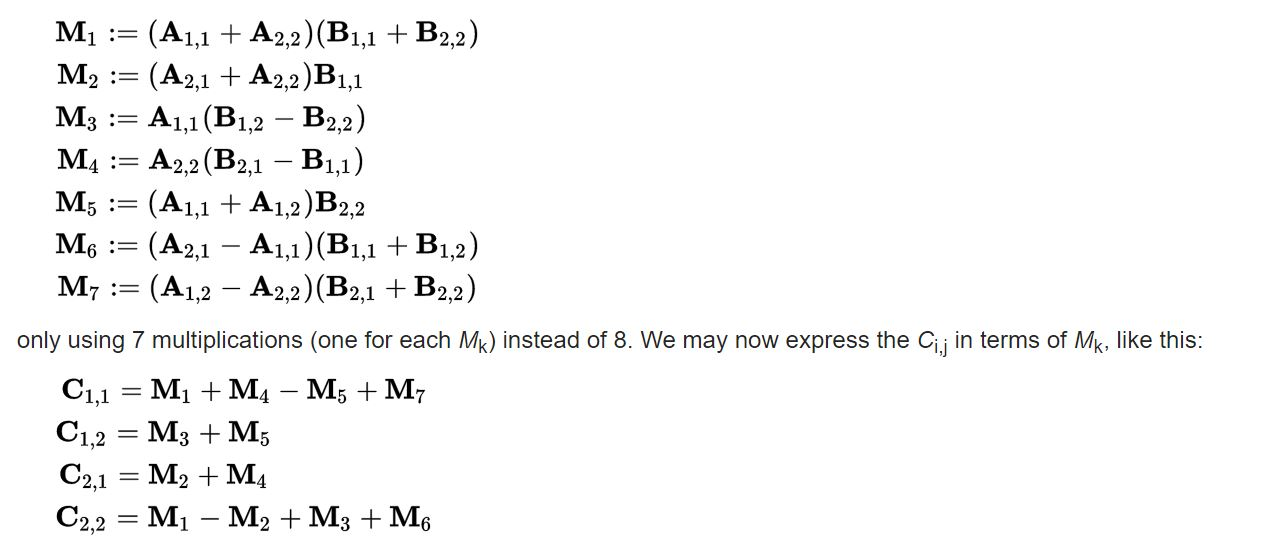
\includegraphics [scale = 0.4] {strassen} \\
I will use their variable naming scheme, both in my writeup and in my code. $A_{1,1}$ refers to the top right quadrant of $A$, and so on. 

One way to implement this code would be to define every matrix named in the above description, then carry out every computation explicitely. My algorithm sacrifices that readibility in favor of having to define fewer variables (and therefore allocate more space) and copy data from one matrix to another fewer times. I define only 3 intermediate $\frac{n}{2} \times \frac{n}{2}$ matrices, and additionally an $n \times n$ matrix $C$ to store my results. $C$ is ultimately returned. The four submatrices of $C$, and the need to copy their contents into the final $C$, can be entirely eliminated by indexing correctly into $C$ when adding on the various $M$'s.  The other 3 matrices I allocated I called $M_{temp}$, $A_{temp}$, and $B_{temp}$. There is no need to declare 7 matrices to store $M_1 ... M_7$ when one could instead reuse a single matrix $M_{temp}$, calculate its value, add it to the appropriate places in $C$, then reuse it for the next $M$. $A_{temp}$ and $B_{temp}$ contain the appropriate combination of submatrices of $A$ and $B$ that correspond to the $M$ we are currently calculating and saving in $M_{temp}$. It is unneccessary to ever define $A_{1, 1}$, etc. We instead index appropriately into $A$ and $B$ when calculating $A_{temp}$ and $B_{temp}$ respectively. Not defining the 4 submatrices of $A$ and $B$ explicitely saves memory and removes the need to copy all of that data an additional time. 

\subsection*{Padding with Zeroes}
I wanted to avoid creating $(n+1) \times (n+1)$ matrices for odd $n$, then having to recopy their entries into $n \times n$ matrices. I wrote a function elt that takes in a matrix and two integers as arguments. It uses the integers to index into the matrix and return the result if the integers are within bounds. Otherwise, it returns 0. I then called this method instead of directly indexing into a matrix everywhere where there was a possibility of needing padding. 

\subsection*{Other Optimizations}
I/O is expensive, and was taking more time than the algorithm itself in my initial implementation (which read and wrote characters one at a time). I fixed this by using Java's built-in BufferedReader to read in the input, and by building then printing a single string with many linebreaks (meaning there's only a single call to file output). In java, the most efficient way to build a long string is to use the StringBuilder class, since Java replaces strings instead of modifying them by default because it treats strings as immutable objects. 


\section*{Experimental Results for $n_0$}
\subsection*{Testing Correctness}
I used the unused first parameter as input for $n_0$ to determine what the experimental value for the optimal $n-0$ is. The program will default to whatever I determine that value to be if 0 is input for the first parameter (as the problem set description said it would be for grading). I wrote a bash script called check to help me test correctness, that would run the program first on an inputted $n_0 < n$, then on $n_0 > n$, and use the shell diff command to check that their respective outputs are identical. When $n_0 < n$, Strassen's algorithm will be used at least once. When $n_0 > n$, only the traditional matrix multiplication algorithm will be used. Therefore, this process checks my implementation of Strassen's algorithm against the traditional matrix multiplication algorithm. 
\subsection*{Runtime for Different $n_0$}
I wrote another bash script called testn0 to experiment efficiently with timing the runtime of different values of $n$ and $n_0$. I was curious if the value of the optimal crossover point might vary with $n$ as well as with $n_0$. It seemed natural to test powers of 2 for $n_0$, and I experimented with several different values of $n$. Changing $n$ slightly did not appear to significantly affect the runtime, nor did the choice of using powers of 2 for $n$ vs other integers. I averaged over 5 trials to reduce statistical variation. The first entry in the table, with $n_0 > n$, represents using the traditional multiplication algorithm.
\begin{center}
\begin{tabular} { |c|c|c| }
\hline
$n$ & $n_0$ & runtime \\
\hline\hline
1000 & $>1000$ & 0.82s \\
\hline\hline
1000 & 64 & 1.38s \\
\hline
1000 & 128 & 0.83s \\
\hline
1000 & 256 & 0.82s \\
\hline
1000 & 512 & 0.67s \\ 
\hline
\end{tabular}
\end{center}
$ n_0 \approx 512$ looks promising. We experiment with a few more values of $n$. 
\begin{center}
\begin{tabular} { |c|c|c| }
\hline
$n$ & $n_0$ & runtime \\
\hline\hline
2000 & $>2000$ & 4.43s \\
\hline\hline
2000 & 64 & 5.36s \\
\hline
2000 & 128 & 3.47s \\
\hline
2000 & 256 & 2.76s\\
\hline
2000 & 512 & 2.77s \\ 
\hline
2000 & 1024 & 3.83s\\
\hline
\end{tabular}
\end{center}

\begin{center}
\begin{tabular} { |c|c|c| }
\hline
$n$ & $n_0$ & runtime \\
\hline\hline
1500 & $>1500$ & 2.11s \\
\hline\hline
1500 & 64 & 2.72 s \\
\hline
1500 & 128 & 2.10s \\
\hline
1500 & 256 & 1.68s\\
\hline
1500 & 512 & 1.45s \\ 
\hline
1500 & 1024 & 1.78s\\
\hline
\end{tabular}
\end{center}

\begin{center}
\begin{tabular} { |c|c|c| }
\hline
$n$ & $n_0$ & runtime \\
\hline\hline
2500 & $>2500$ & 8.80 s \\
\hline\hline
2500 & 64 &  13.59 s \\
\hline
2500 & 128 & 8.60 s \\
\hline
2500 & 256 &  6.85 s\\
\hline
2500 & 512 & 6.33 s \\ 
\hline
2500 & 1024 & 5.40 s\\
\hline
\end{tabular}
\end{center}

$n_0 = 512$ seems to be producing the best result, ie to use Strassen's algorithm for $n \geq 512$ and not use Strassen's algorithm for $n < 512$. This is much higher than the values for $n_0$ that my classmates seemed to be getting. I am convinced that the majority of the difference comes not from slowness in my Strassen's algorithm, but from the optimizations I did for my naive multiplication algorithm. Not only did I rearrange the matrix order as suggested, but I also saved some intermediate values (discussed above). Saving intermediate values speeds up the naive multiplication algorithm by an additional factor of 2-3 in my tests, which has the consequence of pushing $n_0$ much higher than it would be if I disabled that. In fact, when I commented out that additional caching optimization, I found that it was optimal to use the Strassen's algorithm for $n=128$, and to start using the conventional algorithm at $n=64$. 

This table gives results for $n_0$ with the correct $i$, $k$, $j$ ordering but without the additional caching optimization on the naive algorithm.
\begin{center}
\begin{tabular} { |c|c|c| }
\hline
$n$ & $n_0$ & runtime \\
\hline\hline
1024 & $>1024$ &  1.9 s\\
\hline\hline
1024 & 32 & 1.8 s \\
\hline
1024 & 64  & 1.6 s \\
\hline
1024 & 128 & 1.4 s\\
\hline
1024 & 256 & 1.5 s\\
\hline
1024 & 512 & 1.5 s \\ 
\hline
1024 & 1024 & 1.6 s\\
\hline
\end{tabular}
\end{center}
In this implementation (since $n$ is a power of 2 and the program executes Strassen's algorithm if $n = n_0$), the last time Strassen's algorithm is used should be at either $n=128$, with the naive algorithm beginning at $n=64$.

\section*{Theoretical Results for $n_0$} 
\subsection*{Recurrence Relation Calculations}
The conventional algorithm has runtime $T_C (n) = 2 n^3$. This is because the innermost for loop performs 2 operations: the multiplication a[i][k] * b[k][j] and incrementing j to iterate through the innermost for loop. 

To calculate the theoretical runtime $T_S(n)$ of Strassen's algorithm, we break it into steps. 

Recursively calling multiply($A_{temp}$, $B_{temp}$) takes $\min(T_S(\frac{n}{2}), T_C(\frac{n}{2}))$ time. At $n=n_0$, it will be optimal to use the conventional algorithm in our recursion, and so calling multiply will take $T_C(\frac{n_0}{2}) = \frac{1}{4} n_0^3$ time. This operation is performed once for each $M$, for a total of 7 times. 

The other steps performed in Strassen's algorithm are as follows, with the cost of incrementing the counter on the innermost for loop variable included for each nested for loop. Steps that are $o(n^2)$ are omitted. \\\\
calculate input to M1: $7n^2$\\
add M1 to C: $7 n^2$\\
calculate input to M2: $5n^2$\\
add M2 to C: $9n^2$\\
calculate input to M3: $5n^2$\\
add M3 to C: $9 n^2$\\
calculate input to M4: $5n^2$\\
add M4 to C: $5n^2$\\
calculate input to M5: $5n^2$\\
add M5 to C: $5 n^2$\\
calculate input to M6: $5 n^2$\\
add M6 to C: $6 n^2$\\
calculate input to M7: $9 n^2$\\
add M7 to C: $2n^2$

In total, $T_S(n) = 84 n^2 + 7 \min(T_S(\frac{n}{2}), T_C(\frac{n}{2}))$. It follows that $T_S(n_0) = 84 n_0^2 + \frac{7}{4} n_0^3$. We find our theoretical value of $n_0$ by setting $T_S(n_0) = T_C (n_0)$, which yields $n_0 = 336$. This is reasonably close to the values we found for $n_0$ experimentally, especially given how much we have found the details of the implementation affects performance via caching. 

\subsection*{Compiler Optimization and Theoretical Runtime}
In the previous section, we found our theoretical $n_0 = 336$. This is higher than it strictly needs to be, given our methodology for calculating theoretical runtime. For example, there are several places with lines of code inside 2 nested for loops similar to

\begin{verbatim}
a_temp[i][j] = elt(a, i, j + n2) - elt(a, i + n2, j + n2);
b_temp[i][j] = elt(b, i + n2, j) + elt(b, i + n2, j + n2);
\end{verbatim}

My analysis counted each computation of i + n2 and j + n2 as a separate operation, with each contributing an addition 1 unit of time cost. This prompted me to experiment with whether recomputing i + n2 and j + n2 actually slows down my algorithm by any noticeable constant factor. It doesn't. I suspect this is because of compiler optimization and how it interacts with assembly. I remember from CS61 examples of assembly saving the result of a simple computation in a register then retrieving that value from the register multiple times instead of redoing the computation multiple times. This is good, because I think the code is a lot more readable with i + n2 and j + n2 written out each time instead of saving those computations in an intermediate variable each time.  I also remember that even very simple programs produced cryptic assembly code, so I did not attempt to verify this explicitely by actually examining the assembly. Reperforming the analysis in the previous section but assuming that i + n2 and j + n2 are not recomputed within a single iteration of the innermost for loop (or, if you prefer, rewriting the code to explicitly store the values of i + n2 and j + n2 then computing the theoretical analysis), gives:\\\\
calculate input to M1: $7n^2$\\
add M1 to C: $7 n^2$\\
calculate input to M2: $5n^2$\\
add M2 to C: $9n^2$\\
calculate input to M3: $5n^2$\\
add M3 to C: $9 n^2$\\
calculate input to M4: $5n^2$\\
add M4 to C: $5n^2$\\
calculate input to M5: $5n^2$\\
add M5 to C: $5 n^2$\\
calculate input to M6: $5 n^2$\\
add M6 to C: $6 n^2$\\
calculate input to M7: $9 n^2$\\
add M7 to C: $2n^2$

This analysis gives $T_{S'}(n) = 60 n^2 + 7 \min(T_S'(\frac{n}{2}), T_C(\frac{n}{2}))$. It follows that $T_{S'} (n_0) = 60 n_0^2 + \frac{7}{4} n_0^3$. Setting this equal to $T_C(n_0) = 2 n_0^3$ and solving for $n_0$ as before gives $n_0 = 240$. 






\end{document}
